\documentclass{article}

\usepackage{fancyhdr}
\usepackage{extramarks}
\usepackage{amsmath}
\usepackage{amsthm}
\usepackage{amsfonts}
\usepackage{tikz}
\usepackage[plain]{algorithm}
\usepackage{algpseudocode}
\usepackage{dsfont}
\usepackage{subcaption}
\usepackage{lipsum}
\usepackage{ragged2e}

\usetikzlibrary{automata,positioning}

%
% Basic Document Settings
%

\usepackage{graphicx, url}
\graphicspath{figures/}

\topmargin=-0.45in
\evensidemargin=0in
\oddsidemargin=0in
\textwidth=6.5in
\textheight=9.0in
\headsep=0.25in

\linespread{1.1}

\pagestyle{fancy}

% The page Header
\lhead{\hmwkAuthorName}
\chead{\hmwkClassShort}
\rhead{\hmwkTitle}
\lfoot{\lastxmark}
\cfoot{\thepage}

\renewcommand\headrulewidth{0.4pt}
\renewcommand\footrulewidth{0.4pt}

\setlength\parindent{0pt}

%
% Create Problem Sections
%

\newcommand{\enterProblemHeader}[1]{
    \nobreak\extramarks{}{Problem \arabic{#1} continued on next page\ldots}\nobreak{}
    \nobreak\extramarks{Problem \arabic{#1} (continued)}{Problem \arabic{#1} continued on next page\ldots}\nobreak{}
}

\newcommand{\exitProblemHeader}[1]{
    \nobreak\extramarks{Problem \arabic{#1} (continued)}{Problem \arabic{#1} continued on next page\ldots}\nobreak{}
    \stepcounter{#1}
    \nobreak\extramarks{Problem \arabic{#1}}{}\nobreak{}
}

\setcounter{secnumdepth}{0}
\newcounter{partCounter}
\newcounter{homeworkProblemCounter}
\setcounter{homeworkProblemCounter}{1}
\nobreak\extramarks{Problem \arabic{homeworkProblemCounter}}{}\nobreak{}

%
% Homework Problem Environment
%
% This environment takes an optional argument. When given, it will adjust the
% problem counter. This is useful for when the problems given for your
% assignment aren't sequential. See the last 3 problems of this template for an
% example.
%
\newenvironment{homeworkProblem}[1][-1]{
    \ifnum#1>0
        \setcounter{homeworkProblemCounter}{#1}
    \fi
    \section{Problem \arabic{homeworkProblemCounter}}
    \setcounter{partCounter}{1}
    \enterProblemHeader{homeworkProblemCounter}
}{
    \qed
    \exitProblemHeader{homeworkProblemCounter}
}

%
% Homework Details
%   - Title
%   - Due date
%   - Class
%   - Section/Time
%   - Instructor
%   - Author
%

\newcommand{\hmwkTitle}{Homework 1}
\newcommand{\hmwkDueDate}{April, 19}
\newcommand{\hmwkClassShort}{AMATH 563 }
\newcommand{\hmwkClass}{\hmwkClassShort \\ Inferring Structure of Complex Systems}
\newcommand{\hmwkClassTime}{Section A}
\newcommand{\hmwkClassInstructor}{Prof. J. Nathan Kutz}
\newcommand{\hmwkAuthorName}{\textbf{Alexey Sholokhov}}
\newcommand{\hmwkAuthorEmail}{\textit{aksh@uw.edu}}
\newcommand{\hmwkAbstract}{In this assignment we work study the behavior of the linear regression solvers on a multiclass image classification data. We show that there is an optimal balance between classifiers complexity and accuracy. We use sparsity promotion properties of LASSO to rank pixels by their importance for classification.}

%
% Title Page
%

\title{
    \vspace{2in}
    \textmd{\textbf{\hmwkClass\\\ \hmwkTitle}}\\
    \normalsize\vspace{0.1in}\small{Due\ on\ \hmwkDueDate\ at 23:59}\\
    \vspace{0.1in}\large{\textit{\hmwkClassInstructor}}
    \vspace{1in}\\
    \justify{\textbf{Abstract: }\hmwkAbstract}
    \vspace{1in}
}


\author{\hmwkAuthorName\\ \hmwkAuthorEmail}
\date{\today}

\renewcommand{\part}[1]{\textbf{\large Part \Alph{partCounter}}\stepcounter{partCounter}\\}

%
% Various Helper Commands
%

% Useful for algorithms
\newcommand{\alg}[1]{\textsc{\bfseries \footnotesize #1}}

% For derivatives
\newcommand{\deriv}[1]{\frac{\mathrm{d}}{\mathrm{d}x} (#1)}

% For partial derivatives
\newcommand{\pderiv}[2]{\frac{\partial}{\partial #1} (#2)}

% Integral dx
\newcommand{\dx}{\mathrm{d}x}

% Alias for the Solution section header
\newcommand{\solution}{\paragraph{Solution} }

% Probability commands: Expectation, Variance, Covariance, Bias
\newcommand{\Var}{\mathrm{Var}}
\newcommand{\Cov}{\mathrm{Cov}}
\newcommand{\Bias}{\mathrm{Bias}}
\newcommand*{\pd}[3][]{\ensuremath{\frac{\partial^{#1} #2}{\partial #3}}}
\newcommand*{\prob}[1]{\ensuremath{\mathbb{P}\left[#1\right]}}
\newcommand*{\ind}[1]{\ensuremath{\mathds{1}_{\left[#1\right]}}}
\newcommand*{\at}[2]{\Big|_{#1}^{#2}}

%
% Different math operators
\DeclareMathOperator{\dom}{Dom}
\DeclareMathOperator{\diag}{Diag}
\DeclareMathOperator{\prox}{prox}
\DeclareMathOperator*{\proj}{proj}
\DeclareMathOperator*{\sign}{sign}
\DeclareMathOperator*{\argmax}{argmax}
\DeclareMathOperator*{\argmin}{argmin}

%% \mathbb symbols
\DeclareMathOperator{\E}{\mathbb{E}}
\DeclareMathOperator{\A}{\mathbb{A}}
\DeclareMathOperator{\R}{\mathbb{R}}
\DeclareMathOperator{\X}{\mathbb{X}}
\DeclareMathOperator{\N}{\mathbb{N}}
\DeclareMathOperator{\Q}{\mathbb{Q}}

%% \mathcal symbols
\DeclareMathOperator{\RR}{\mathcal{R}}
\DeclareMathOperator{\PP}{\mathcal{P}}
\DeclareMathOperator{\NN}{\mathcal{N}}
\DeclareMathOperator{\CC}{\mathcal{C}}
\DeclareMathOperator{\FF}{\mathcal{F}}
\DeclareMathOperator{\YY}{\mathcal{Y}}



\begin{document}

\maketitle
\newpage

\section{Introduction}
Multi-class classification has been a topic of a great attention due to its broad applicability in various domains: from text and image recognition to fundamental physics and behavior prediction. A typical multi-class classification setup denotes a set of objects and a set of classes, each object belongs to one class only. The goal is to approximate an unknown mapping from a feature space to classes within a given family of models in the best way possible. An optimal model is set to be an empirical risk minimizer, where the optimization goes with respect to model parameters. The optimizing function is called a loss function. 

Vast variety of models have been proposed for the multi-class classification problem during the last four decades, including linear models, which are acknowledged for their simplicity and computational performance. The linear regression is the simplest model of this class: answers are considered to be linear combination of features plus Gaussian noise, which appears to be a feasible assumption for many real-world applications. Ridge estimator \cite{ridge} is a second norm regularized linear regression, so the model coefficients are assumed to be of a Gaussian distribution.  LASSO \cite{lasso}, a linear regression with an imposed Laplacian prior on model parameters, is another linear model, which is known for its sparsity promotion capabilities. 

The MINIST dataset is one of the most famous benchmarks for image classification \cite{mnist}. It comprises of 60 thousand hand-written digits naturally divided into 10 classes according to the numbers they represent. 

In this work we apply linear regression models to MINIST in order to find the most informative subset of pixels in general and for each classifier individually. For feature selection we use sparsity promotion property of LASSO.

\section{Theoretical Background}
\paragraph{Notation} Let $\{x_i, y_i\}_{i = 1}^n$ be a set of $n$ training samples, each object $x_i$ is as a real vector of $m$ coordinates: $x_i \in \R^m$, and $y_i \in \YY$ is an object's class label where $\YY$ is a set of all possible labels, $\|\YY\| = k$. Let $A$ be a matrix of objects stacked row-wise, $Y$ be a column of answers labels. Let $X$ be the matrix which $i$'th column is a vector of the model parameters for $i$'th class respectively. We denote $\|X\|_F$ as a Frobenius norm of a matrix $X$, which is a squared root of the sum of its squared elements: $\|X\|_F = \sqrt{\sum_{ij}x_{ij}}$. We define sparsity of a matrix $X$ as a fraction of zero elements in it.

\paragraph{Multi-class classification as a linear regression problem.} We apply one-hot encoding technique for representing the answer set as a set of $k$ vectors containing only one non-zero coordinate each. Precisely 
    \begin{equation}
        \label{eq:ohe_answers}
        B = [y_1, y_2, \dots, y_n], \quad \text{where} \quad y_i = [0, \dots, 1_i, \dots 0]
    \end{equation}
    
    We want to find a matrix $X^* \in R^{m \times k}$ such that that 
    \begin{equation}
        \label{eq:least_squares}
        X^* = \argmax_{X \in R^{m \times k}} \|AX - B\|^2_F
    \end{equation}
    known also as a least squares problem minimizer. Due to the convexity property the problem has a solution.
    In this work we apply four different solvers for this problem:

\begin{enumerate}
    \item \textbf{Pseudoinverse matrix} for matrix A is defined as
        \begin{equation}
            \label{eq:pinverse}
            A^\dag = (A^TA)^{-1}A^T
        \end{equation}
    one may check that 
        \[
            X^* = A^\dag B
        \]
    solves the problem \ref{eq:least_squares}. 
    \item \textbf{Linear regression} is defined as
        \begin{equation}
            \label{eq:linreg}
            \min_{X \in R^{m \times k}} \|AX - B\|^2_F
        \end{equation}
        which is a basic least squares setup with no regularization.
    \item \textbf{Ridge Regression} is defined as 
        \begin{equation}
            \label{eq:ridge}
            \min_{X \in \R^{m \times k}} \|AX - B\|_F^2 + \frac{\lambda}{2}\|x\|_2^2
        \end{equation}
        where $\lambda$ is a regularization coefficient, the second norm regularization is used.
    \item \textbf{LASSO} is defined as 
        \begin{equation}
            \label{eq:lasso}
            \min_{X \in \R^{m \times k}} \|AX - B\|_F^2 + \frac{\lambda}{2}\|x\|_1
        \end{equation}
        where $\lambda$ is the regularization coefficient, the first norm regularization is used. Increasing $\lambda$ encourages the model to use less features hence promotes sparsity for model coefficients. 
\end{enumerate}

\paragraph{Metrics for classification quality} As classes in the dataset are well-balanced, we use the micro-averaged accuracy as a classification quality measure.

\section{Algorithm Implementation and Development}
This section supplements and clarifies the Jupyter notebook attached to this report (see the Appendix B)

\paragraph{Section 1: Reading and preprocessing the data} For interacting with the MINIST dataset the \texttt{minist}  package is used \cite{ministpython}. Train and test objects are stored in the variables \texttt{train\_data} and \texttt{test\_data} respectively. The data and class labels are then preprocessed and reshaped according to the assignment requirements (see the formula \ref{eq:ohe_answers}). No trimming, up- or downsampling, scaling, or any other kind of preprocessing is used.
 
\paragraph{Section 2: Determining the mapping from the image space to the label space} 
    We sequentially apply four solvers listed in the previous section (see equations \ref{eq:pinverse}, \ref{eq:linreg}, \ref{eq:ridge}, \ref{eq:lasso}) to the problem \ref{eq:least_squares}. For measuring classification quality we use the \texttt{sklearn.metrics.accuracy\_score} and \texttt{sklearn.metrics.classification\_report} functions (see Appendix A and \cite{classificationreport} for references). In this section default parameters were used ($\lambda = 1$ for Ridge and Lasso) for all the algorithms, no extra tuning was made.
\paragraph{Section 3: Feature selection via sparsity promotion} We use the LASSO algorithm for building sparse linear models. For each $\lambda \in [0, 0.1, \dots 9.9, 10]$ a LASSO model is generated, all the models coefficients are stored in the list \texttt{lasso\_models}. For each model, classification accuracy, sparsity and the coefficients importance were calculated, they are plotted in the figure \ref{fig:important_pixels} (the discussion is in the next section). Finally, all the models coefficients were extracted  and stored as the \texttt{coefs} array. 

    We say that a pixel is important to a classifier if there is at least one class which linear model uses this pixel in prediction (the respective coefficient is not zero). A matrix named \texttt{important\_pixels} was filled according to this principle: each column $i$ of the matrix is a binary array, which marks all the pixels which are used by the LASSO model with a given $\lambda_i$. This array is displayed in the figure \ref{fig:important_pixels}. 
    
\paragraph{Section 4: Establishing sets of important pixels for individual classifiers.} Similarly to the previous section, a set of LASSO models with different $\lambda$ was generated, but now for each of 10 classes a classifier was build separately. All the coefficients of these classifiers were stored into the \texttt{ind\_coefficients} array. 

Finally, important pixels depending on the regularization coefficient are displayed atop of sample pictures from the dataset (see the figure \ref{fig:pixels_with_background}). 
    

\section{Computational Results}

\begin{table}
    \centering
    \label{table:classification_quality}
    \begin{tabular}{l||c|c|c|c||}
         & Precision & Recall & F1-score & Sparsity \\
         \hline \hline 
         Pseudoinverse & 0.85 & 0.85 & 0.85 &  0.02 \\
         \hline
         Linear Regression & 0.86 & 0.86 & 0.86 & 0.02 \\
         \hline
         Lasso & 0.83 & 0.83 & 0.83 & \textbf{0.89} \\
         \hline
         Ridge & 0.86 & 0.86 & 0.86 & 0.08 \\
         \hline 
    \end{tabular}
    \caption{Classification scores for different linear regression solvers. All of them have similar accuracy, yet LASSO provides significantly more sparse solution than other competitors.}
\end{table}


\begin{figure}
    \label{fig:important_pixels}
    \centering
    \includegraphics[width=0.8\textwidth]{images/important_pixels}
    \caption{The importance of pixels is shown at the upper-left figure. For each pixel the corresponding blue line indicates for how long this pixel had a non-zero coefficient in the model. Top-100 important pixels are marked with red, they are illustrated on the bottom-right part of the image. The accuracy and sparsity plots are in the bottom-left part of the picture, the x-axis is shared for all three plots. The top-12 important pixels coordinates are listed on the right.}
\end{figure}

\begin{figure}[t!]
    \label{fig:important_pixels}
    \begin{subfigure}[t!]{0.65\textwidth}
        \centering
        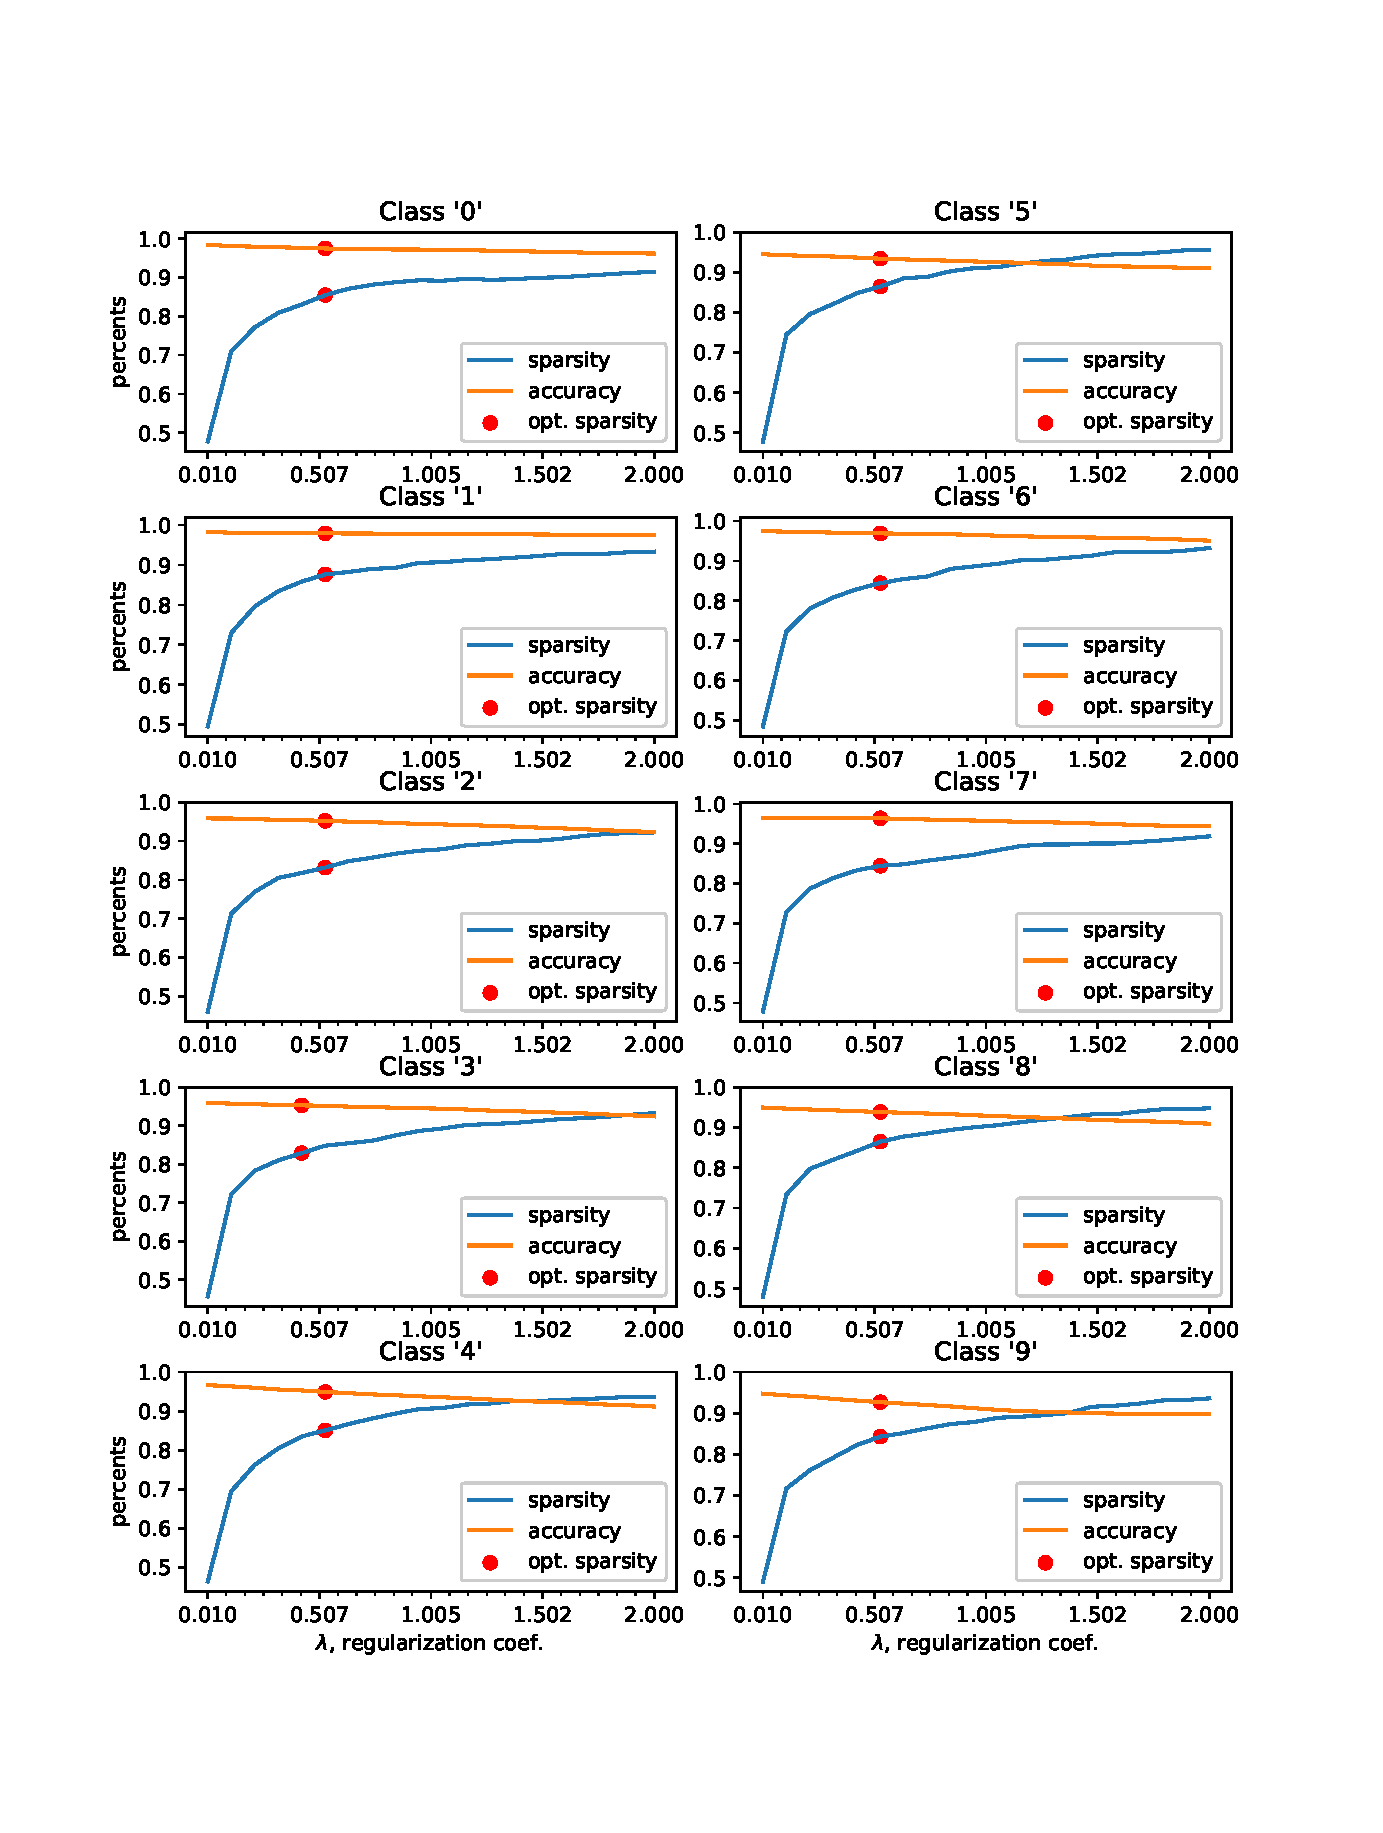
\includegraphics[width=\textwidth]{images/classifiers_ind_sparsity}
        \caption{Plots of sparsity vs accuracy for each classifier built individually. }
    \end{subfigure}%
    \begin{subfigure}[t!]{0.40\textwidth}
        \centering
        \begin{subfigure}{\textwidth}
            \centering
            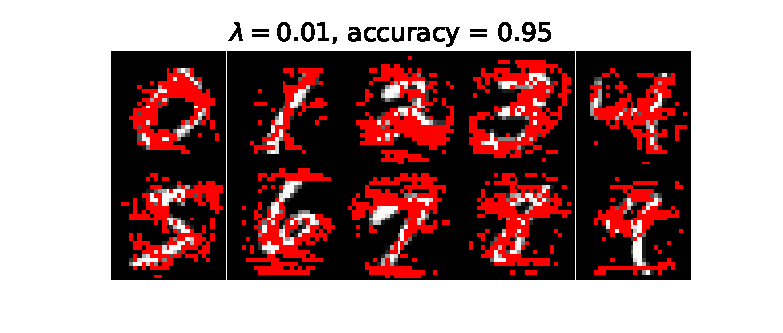
\includegraphics[width=\textwidth]{images/pixels_with_background_0}
        \end{subfigure}
        \begin{subfigure}{\textwidth}
            \centering
            \includegraphics[width=\textwidth]{images/pixels_with_background_1}
        \end{subfigure}
        \begin{subfigure}{\textwidth}
            \centering
            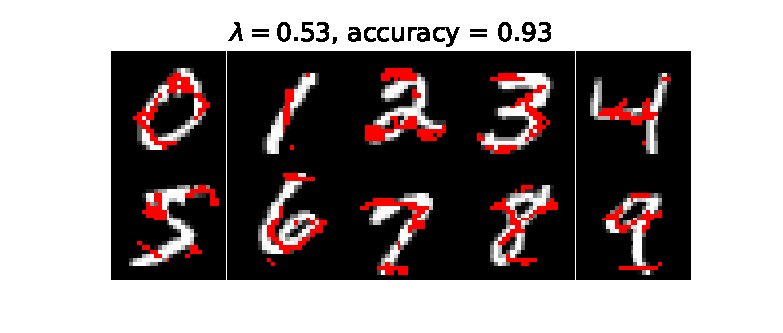
\includegraphics[width=\textwidth]{images/pixels_with_background_2}
        \end{subfigure}
        \begin{subfigure}{\textwidth}
            \centering
            \includegraphics[width=\textwidth]{images/pixels_with_background_3}
        \end{subfigure}
        \caption{Important pixels (red) on sample pictures depending on the regularization coefficient. The third set corresponds to the optimal sparsity level.}
    \end{subfigure}
    \caption{The optimal point, the steep slope criteria, is almost the same to all classifiers, although sparsity increases with different rate.}
\end{figure}


In this section we discuss the computational results
\paragraph{Problem 1} The classification quality for the four linear regression solvers are listed in the Table \ref{table:classification_quality}. All of them have similar accuracy, yet LASSO provides significantly more sparse solution.

\paragraph{Problem 2} We use LASSO for finding and ranking pixels which are  important for classification. Precisely, we gradually increase the regularization coefficient $\lambda$ and for each pixel we check when the respective coefficient goes to zero, simultaneously measuring classification quality. The figure \ref{fig:important_pixels} illustrates this experiment. We see that there is a steep slope in sparsity around $\lambda = 0.4$: before this point the algorithm nullifies almost 90\% of its coefficients without significant drop in quality, but after this point losing pixels proportionally decreases the classification accuracy. This experiment also allows us to rank pixels according to its importance: the more important the pixel is -- the longer the respective coefficient remains nonzero (which corresponds to the length of its blue line on the figure \ref{fig:important_pixels}). The top 15 pixels, sorted by their importance, is listed on the right part of the figure \ref{fig:important_pixels}, the top-100 important pixels are displayed on the bottom-rightmost cell. 

\paragraph{Problem 3} The optimal value $\lambda = 0.4$ gives the classification accuracy \textbf{0.85} while having only 17\% non-zero coefficients. This accuracy matches with the accuracy from other methods (see the Table \ref{table:classification_quality}) with almost fully dense coefficient matrices. It means, that the remaining pixels carry the majority of useful information and can be defined as the important features subset.

\paragraph{Problem 4} We then redo the previous experiment for each classifier separately, the results are presented on the Figure \ref{fig:individual_pixels}. We see that optimal sparsity does not vary significantly for different classifiers, although sparsity increases with slightly different rate.

 Finally the most important pixels for different lambdas for each classifier are displayed on the Figure \ref{fig:important_pixels_with_background}. We see that for $\lambda = 0.53$ the important pixels sets clearly match with the natural intuition and expectations.
 
 \paragraph{Problem 5} When we are doing the $AX=B$ fitting, we are essentially building $k$ linear classifiers for each class: they learn to predict 1 for objects of their class and 0 otherwise.
    
    
    
\section{Summary and Conclusion}
In this work we worked with linear models in multiclass classification setup. We learned that LASSO is a useful tool for feature selection and sparsity promotion purposes. We also learned how to find an optimal balance between model simplicity and classification accuracy.  


\begin{thebibliography}{99}

\bibitem{ministpython} \url{https://github.com/datapythonista/mnist}
\bibitem{classificationreport} \url{https://scikit-learn.org/stable/modules/generated/sklearn.metrics.classification_report.html}
\bibitem{ridge}Tikhonov, Andreï Nikolaevitch, et al. Numerical methods for the solution of ill-posed problems. Vol. 328. Springer Science \& Business Media, 2013
\bibitem{lasso}Tibshirani, Robert. "Regression shrinkage and selection via the lasso." Journal of the Royal Statistical Society: Series B (Methodological) 58.1 (1996): 267-288.
\bibitem{mnist}LeCun, Yann, Corinna Cortes, and C. J. Burges. "MNIST: handwritten digit database." AT\&T Labs [Online]. Available: \url{http://yann.lecun.com/exdb/mnist}
\end{thebibliography}

\newpage

\section{Appendix A}
Besides the standard classes and the \texttt{pylab} environment functions. the following python functions were used:
\begin{enumerate}
    \item \texttt{sklearn.linear\_model.LinearRegression} implements a simple nonregularized linear regression, see \url{https://scikit-learn.org/stable/modules/generated/sklearn.linear_model.LinearRegression.html}
    \item \texttt{sklearn.linear\_model.Lasso} implements a LASSO regression (equation \ref{eq:lasso}), see \url{https://scikit-learn.org/stable/modules/generated/sklearn.linear_model.Lasso.html}
    \item \texttt{sklearn.linear\_model.Ridge} implements a Ridge regression (equation \ref{eq:ridge}), see \url{https://scikit-learn.org/stable/modules/generated/sklearn.linear_model.Ridge.html}
    \item \texttt{sklearn.metrics.classification\_report} provides a neat report of different classification metrics (precision, recall, f1-measure) see \url{https://scikit-learn.org/stable/modules/generated/sklearn.metrics.classification_report.html}
    \item \texttt{sklearn.metrics.accuracy\_score} calculates the classification acuracy, see \url{https://scikit-learn.org/stable/modules/generated/sklearn.metrics.accuracy_score.html}
\end{enumerate}
\end{document}
